\documentclass[14pt,xcolor=dvipsnames,pdftex]{beamer}
\usepackage[utf8x]{inputenc}
\usepackage[T1]{fontenc}
\usepackage[ngerman]{babel}
\usepackage{hyperref}
\usepackage{pgfpages}
\usepackage{color}
\usepackage{textcomp}
\usepackage{alltt}
\usepackage{amsmath}
\usepackage{amsfonts}
\usepackage{booktabs}

\usepackage{inconsolata} % TT font
\usepackage{array}
\usepackage{url}
%\usepackage[svgnames]{xcolor}\\
%\usetheme[secheader]{Boadilla}
%\usefonttheme{sans}
\setbeamersize{text margin left=1cm,text margin right=1cm}
\setbeamertemplate{section in toc}[Palo Alto]

\newcolumntype{T}{c<{\ttfamily}}

\title{Textkompression: Burrows-Wheeler-Transformation}
\subtitle{Proseminar \glqq Algorithmen der Bioinformatik\grqq}
\author{Uli Köhler}
\date{12.~November 2012}

\setbeamertemplate{footline}
{%
%\begin{beamercolorbox}[wd=0.5\textwidth,ht=3ex,dp=1.5ex,leftskip=.5em,rightskip=.5em]{author in head/foot}%
%\usebeamerfont{author in head/foot}%
%\insertframenumber\hfill\insertshortauthor%
%\end{beamercolorbox}%
\vspace*{-4.5ex}\hspace*{0.5\textwidth}%
\begin{beamercolorbox}[width=\textwidth,ht=3ex,dp=1.5ex,left]{title in head/foot}%
\usebeamerfont{title in head/foot}%
Folie \insertframenumber{} von \inserttotalframenumber\hspace{8mm}
%\insertshorttitle%
\end{beamercolorbox}%
}

\AtBeginSection[]{} % for optional outline or other recurrent slide

\begin{document}
\frame{\titlepage}
\begin{frame}
\frametitle{Aufbau dieser Präsentation}
\begin{itemize}
 \item Kompression in der Bioinformatik
 \item Die Burrows-Wheeler-Transformation
 \begin{itemize}
  \item Algorithmus der Hintransformation
  \item Algorithmus der Rücktransformation
  \item Probleme der BWT
 \end{itemize}
 \item Diskussion verschiedener Resultate
 \begin{itemize}
  \item Burrows \& Wheeler
  \item Cox \& Bauer
  \item Eigene Resultate
 \end{itemize}


\end{itemize}

\end{frame}

%%%%%%% Compression basics
\section{Grundlagen der Datenkompression}
\begin{frame}[allowframebreaks]
\frametitle{Große Datenmengen in der Bioinformatik}
  \begin{itemize}
   \item High-Throughput-Sequencing erzeugt durch \textit{n}-fache Abdeckung große Datenmengen
   \item Oft Speicherung der Rohdaten gewünscht
   \item Speicherplatz ist teuer, teils langsamer Zugriff
\end{itemize}
\framebreak
\begin{itemize}
 \item \textbf{Lösung:} Verlustfreie Datenkompression\\
 \textrightarrow\ Daten unter Einsatz von weniger\\
 \quad\ Speicherplatz darstellen
 \item Prinzip: Eliminierung von Redundanzen
 \item Anforderungen je nach Anwendung:
 \begin{itemize}
  \item Schnelle Kompression/Dekompression
  \item Wenig Speicherplatzverbrauch
 \end{itemize}
\end{itemize}
\end{frame}
%%%%%% Naive algorithm
\begin{frame}[allowframebreaks]
\frametitle{Ein naiver Kompressionsalgorithmus}
\begin{itemize}
 \item Eingabestring $S := AAAAAAAAATTT$ \textrightarrow $|S| = 12$
 \item Der 	Algorithmus fasst gleiche aufeinanderfolgende Zeichen (\textit{Runs}) zusammen
 \item Resultat: $S' = $ 9A3T \textrightarrow $|S'|$ = 4\\	\textrightarrow\ 75\% Speicherplatzeinsparung
 \item Problem: Viele Strings (z.B. \texttt{ATATATAT}) können nicht komprimiert werden
\end{itemize}
\framebreak
\begin{itemize}
 \item Aufeinanderfolgende gleiche Zeichen können von diesem Algorithmus besser komprimiert werden
 \item Einige reale Kompressionsalgorithmen können davon ebenfalls profitieren
 \item Ist es möglich, einen String \textit{reversibel} so umzuordnen, dass möglichst viele, möglichst lange \textit{Runs} auftreten?\\
 \textrightarrow\ \textbf{Burrows-Wheeler-Transformation}
\end{itemize}
\end{frame}

\section{Burrows-Wheeler-Transformation}
%%%%%% 	
\subsection{Algorithmus der Burrows-Wheeler-Transformation}
\begin{frame}[allowframebreaks]
 \frametitle{BWT - Kompression}
    \begin{columns}[c,onlytextwidth]
    \column{0.55\textwidth}
    \begin{itemize}
	\item Eingabestring $S := \text{\texttt{aabrac}}$	
	\item Initialisierung einer Matrix M der Dimensionen $|S| \times |S|$
	\item Bildung aller zyklischen Rotationen des Eingabestrings
    \end{itemize}
    \column{0.45\textwidth}
    \begin{center}
    \begin{tabular}{T|T}
    \multicolumn{2}{c}{\textbf{M}}\\
    0 & aabrac \\
    1 & abraca \\
    2 & bracaa \\
    3 & racaab \\
    4 & acaabr \\
    5 & caabra \\
    \end{tabular}
    \end{center}
    \end{columns}
\framebreak
%%%%%% Sorting
\begin{columns}[c,onlytextwidth]
 \column{.55\textwidth}
 \begin{itemize}
  \item Lexikographische Sortierung der Rotationen des Eingabestrings
 \end{itemize}
 \column{.45\textwidth}
    \begin{tabular}{T}
    \textbf{M} \\
    aabrac \\
    abraca \\
    acaabr \\
    bracaa \\
    caabra \\
    racaab \\
    \end{tabular}
\end{columns}
\framebreak
%%% Output of compression algorithm
\begin{columns}[c,onlytextwidth]
 \column{.55\textwidth}
 \begin{itemize}
  \item Resultat:\\
      Das Tupel \textit{$(L,I)$}, wobei L die {\color{red}letzte Spalte} der Matrix ist
      und I der Index des {\color{blue}Eingabestrings in der Matrix} ist
  \item $(L,I) = (caraab, 1)$
 \end{itemize}
 \column{.45\textwidth}
 \begin{center}
    \begin{tabular}{T|T}
    \multicolumn{2}{c}{\textbf{M}}\\
    0 & aabra{\color{red}c} \\
    {\color{blue}1} & {\color{blue}abrac}{\color{red}a} \\
    2 & acaab{\color{red}r} \\
    3 & braca{\color{red}a} \\
    4 & caabr{\color{red}a} \\
    5 & racaa{\color{red}b} \\
    \end{tabular}
    \end{center}
\end{columns}
\end{frame}
%%%%%% Decompression
\subsection{BWT -- Rücktransformation}
\begin{frame}[allowframebreaks]
\frametitle{BWT -- Rücktransformation}
\begin{columns}[c,onlytextwidth]
 \column{.65\textwidth}
 \begin{itemize}
  \item Eingabetupel: $(L,I)$
  \item Initialisierung einer Matrix M der Dimensionen $|L| \times |L|$
  \item Bereits bekannt: L ist die {\color{blue}letzte Spalte} von M
 \end{itemize}
 \column{.35\textwidth}
    \begin{tabular}{T}
    \textbf{M} \\
    \_\_\_\_\_{\color{blue}c} \\
    \_\_\_\_\_{\color{blue}a} \\
    \_\_\_\_\_{\color{blue}r} \\
    \_\_\_\_\_{\color{blue}a} \\
    \_\_\_\_\_{\color{blue}a} \\
    \_\_\_\_\_{\color{blue}b}
    \end{tabular}
\end{columns}
\framebreak
\begin{columns}[c,onlytextwidth]
 \column{.65\textwidth}
 \begin{itemize}
  \item Die {\color{blue}erste Spalte} ist immer sortiert
  \textrightarrow\ Kann durch sortieren von $L$ ausgefüllt werden
 \end{itemize}

 \column{.35\textwidth}
    \begin{tabular}{T}
    \textbf{M} \\
    {\color{blue}a}\_\_\_\_c\\
    {\color{blue}a}\_\_\_\_a\\
    {\color{blue}a}\_\_\_\_r\\
    {\color{blue}b}\_\_\_\_a\\
    {\color{blue}c}\_\_\_\_a\\
    {\color{blue}r}\_\_\_\_b\\
    \end{tabular}
\end{columns}
\framebreak
\begin{columns}[c,onlytextwidth]
 \column{.65\textwidth}
 \begin{itemize}
  \item Die entstandene Matrix wird um ein Zeichen rotiert
 \end{itemize}
 \column{.35\textwidth}
 \begin{tabular}{T}
    \textbf{M} \\
    \_\_\_\_c{\color{blue}a}\\
    \_\_\_\_a{\color{blue}a}\\
    \_\_\_\_r{\color{blue}a}\\
    \_\_\_\_a{\color{blue}b}\\
    \_\_\_\_a{\color{blue}c}\\
    \_\_\_\_b{\color{blue}r}
  \end{tabular}
\end{columns}
\framebreak
\begin{columns}[c,onlytextwidth]
 \column{.65\textwidth}
 \begin{itemize}
  \item Die Matrix wird lexikographisch sortiert
 \end{itemize}
 \column{.35\textwidth}
 \begin{tabular}{T}
    \textbf{M} \\
    \_\_\_\_aa\\
    \_\_\_\_ab\\
    \_\_\_\_ac\\
    \_\_\_\_br\\
    \_\_\_\_ca\\
    \_\_\_\_ra
  \end{tabular}
\end{columns}
\framebreak
\begin{itemize}
 \item Die Schritte
 \begin{itemize}
  \item Schreiben von L in die rechteste freie Spalte
  \item Lexikographisches Sortieren
 \end{itemize}
 werden wiederholt bis die Matrix voll ist
\end{itemize}
%Demo frames
\framebreak
\begin{columns}
 \column{0.2\textwidth}
 \begin{tabular}{T}
    \textbf{M} \\
    \_\_\_{\color{red}c}aa\\
    \_\_\_{\color{red}a}ab\\
    \_\_\_{\color{red}r}ac\\
    \_\_\_{\color{red}a}br\\
    \_\_\_{\color{red}a}ca\\
    \_\_\_{\color{red}b}ra
  \end{tabular}
 \column{0.1\textwidth}
 $\xrightarrow{\text{Sortieren}}$
 \column{0.4\textwidth}
 \begin{tabular}{T}
    \textbf{M} \\
    \_\_\_aab\\
    \_\_\_abr\\
    \_\_\_aca\\
    \_\_\_bra\\
    \_\_\_caa\\
    \_\_\_rac
  \end{tabular}
\end{columns}
% Demo 2
\framebreak
\begin{columns}
 \column{0.2\textwidth}
 \begin{tabular}{T}
    \textbf{M} \\
    \_\_{\color{red}c}aab\\
    \_\_{\color{red}a}abr\\
    \_\_{\color{red}r}aca\\
    \_\_{\color{red}a}bra\\
    \_\_{\color{red}a}caa\\
    \_\_{\color{red}b}rac
  \end{tabular}
 \column{0.1\textwidth}
 $\xrightarrow{\text{Sortieren}}$
 \column{0.4\textwidth}
 \begin{tabular}{T}
    \textbf{M} \\
    \_\_aabr\\
    \_\_abra\\
    \_\_acaa\\
    \_\_brac\\
    \_\_caab\\
    \_\_raca
  \end{tabular}
\end{columns}
% Demo 3
\framebreak
\begin{columns}
 \column{0.2\textwidth}
 \begin{tabular}{T}
    \textbf{M} \\
    \_{\color{red}c}aabr\\
    \_{\color{red}a}abra\\
    \_{\color{red}r}acaa\\
    \_{\color{red}a}brac\\
    \_{\color{red}a}caab\\
    \_{\color{red}b}raca
  \end{tabular}
 \column{0.1\textwidth}
 $\xrightarrow{\text{Sortieren}}$
 \column{0.4\textwidth}
 \begin{tabular}{T}
    \textbf{M} \\
    \_aabra\\
    \_abrac\\
    \_acaab\\
    \_braca\\
    \_caabr\\
    \_racaa
  \end{tabular}
\end{columns}
% Demo 4
\framebreak
\begin{columns}
 \column{0.2\textwidth}
 \begin{tabular}{T}
    \textbf{M} \\
    {\color{red}c}aabra\\
    {\color{red}a}abrac\\
    {\color{red}r}acaab\\
    {\color{red}a}braca\\
    {\color{red}a}caabr\\
    {\color{red}b}racaa
  \end{tabular}
 \column{0.1\textwidth}
 $\xrightarrow{\text{Sortieren}}$
 \column{0.4\textwidth}
 \begin{tabular}{T}
    \textbf{M} \\
    aabrac\\
    abraca\\
    acaabr\\
    bracaa\\
    caabra\\
    racaab
  \end{tabular}
\end{columns}
\framebreak
\begin{columns}
\column{0.6\textwidth}
\begin{itemize}
 \item $M$ wurde vollständig rekonstruiert
 \item Zeile $I$ ist der {\color{red}Originaltext}
\end{itemize}
\column{0.4\textwidth}
\begin{tabular}{c|T}
    \multicolumn{2}{c}{\textbf{M}} \\
    0 & aabrac \\
    {\color{red}1} & {\color{red}abraca}\\
    2 & acaabr \\
    3 & bracaa \\
    4 & caabra \\
    5 & racaab
\end{tabular}
\end{columns}
\end{frame}
\begin{frame}
\frametitle{BWT -- Rücktransformation (Original)}
\begin{itemize}
 \item Besseres Laufzeitverhalten - keine mehrfache Sortierung notwendig
 \item Berechnung von $C_{ch} := $ Anzahl der Zeichen in $L$, die im Alphabet vor $ch$ vorkommen
 \item Berechnung von $P_i := $ Anzahl der Vorkommen von $L_i$ im Präfix von $L$ der Länge $i$
 \item Rekursive Berechnung des Originaltextes S
 \begin{align}
 i_{|L|} &:= I\\
 i_{j-1} &:= P_{i_j} + C_{L_{i_j}}\\
 S_j &:= L_{i+1}
 \end{align}
\end{itemize}
\end{frame}
%% Suffix trees etc.
\begin{frame}
\frametitle{Effiziente Kompression}
\begin{itemize}
\item Die Kompression kann effizient mit \textbf{Suffix Trees} implementiert werden
\item Aber: Suffix Trees sind auf realer Hardware vergleichsweise langsam \\
\textrightarrow\ Lösung: \textbf{Suffix Arrays} \textrightarrow\ Vortrag am 19.11.2012
\end{itemize}
\end{frame}
%%%%%% Why it compresses well
\begin{frame}
 \frametitle{Komprimierbarkeit}
 \begin{itemize}
  \item Einige Zeichenkombinationen tauchen häufiger in Texten auf als andere, z.B. \textit{an} in \textit{and}
  \item Alle Zeilen von $M$, die mit \textit{nd} beginnen, tauchen nacheinander auf (Sortierung)
  \item Durch Rotation ist bei nahezu allen Zeilen, die mit \textit{nd} beginnen, das letzte Zeichen \textit{a}\\
  \textrightarrow\ $L$ enthält viele aufeinanderfolgende \textit{a}
 \end{itemize}
\end{frame}

%%%%%% Problems and solutions
\subsection{Probleme der BWT}
\begin{frame}
 \frametitle{Skalierbarkeit}
 \begin{itemize}
  \item Komplexität der BWT-Transformation ist $\mathcal{O}(n^2)$\\
    \textrightarrow \ Anwendung der BWT auf sehr große Datensätze (z.B. Genome) skaliert nicht
  \item Zeitverbrauch hauptsächlich durch Sortierung\\
  \textrightarrow\ Wahl des Sortieralgorithmus wichtig
  \item Burrows und Wheeler stellen einen für englische Texte optimierten Quicksort vor
  \item Lösung: Unterteilung des Datensatzes in kleinere \textit{Blöcke} - Anwendung der BWT auf diese Blöcke
 \end{itemize}
\end{frame}
\begin{frame}
 \frametitle{Overhead}
 \begin{itemize}
  \item Die Länge des Tupels $(L,I)$ ist insgesamt größer als $|S|$
  \item Genauer Längenunterschied hängt von der Repräsentation von $(L,I)$ ab
  \item Lösung: Anwendung eines Kompressionsalgorithmus, z.B. der \textit{Huffman-Kodierung} auf $(L,I)$
  \item Je nach Kompressionsalgorithmus oft vorherige Anwendung einer Codierung wie der Move-To-Front-Codierung (\textit{MTF})
  \end{itemize}
\end{frame}
%%%%%% Comp
\begin{frame}
 \frametitle{Vergleich mit anderen Algorithmen}
 \begin{columns}[c,onlytextwidth]
  \column{1\textwidth}
    \begin{itemize}
    \item Kompression ist meist ein Kompromiss zwischen Geschwindigkeit und Platzeinsparung
    \item Einige Algorithmen sind für spezielle Datentypen (z.B. Bilder) besser geeignet
    \item Einige Algorithmen (z.B. \textit{bzip2}) benutzen bereits die BWT\\
    \textrightarrow\ Kein Vergleich möglich
    \end{itemize}
  %\column{0.5\textwidth}
  %\begin{tabular}{c}
  %\textbf{Hohe Kompression}\\
  %\textuparrow \textbf{langsam}\\\hline
  %PAQ8\\
  %LZMA/LZMA2\\
  %bzip2\\
  %Deflate\\\hline
  %\textbf{Geringe Kompression}\\
  %\textuparrow \textbf{schnell}
  %\end{tabular}  
 \end{columns}
\end{frame}

\begin{frame}[allowframebreaks]
 \frametitle{Resultate von Burrows \& Wheeler}
 \includegraphics[width=\textwidth]{graph/bw-1.pdf}
 \framebreak\\
 \includegraphics[width=\textwidth]{graph/bw-2.pdf}
 \framebreak\\
 \includegraphics[width=\textwidth]{graph/bw-3.pdf}
\end{frame}
\begin{frame}
 \frametitle{Diskussion der Resultate von Burrows \& Wheeler}
 \begin{itemize}
  \item Zeitdaten sind kritisch zu bewerten - Hardware von 1994
  \item BWT+Huffman: Gute Kompression, aber dennoch akzeptables Verhältnis \textit{Kompression / Zeit}
  \item Beispiele beziehen sich nicht auf Bioinformatik-Datensätze, sondern auf einen Kompressionstestkorpus
 \end{itemize}
\end{frame}
\begin{frame}[allowframebreaks]
 \frametitle{Resultate von Cox \& Bauer}
 \begin{itemize}
  \item BWT muss zur Anwendung von Sequenzdaten generalisiert werden
  \item Cox \& Bauer definieren dafür den BWT-SAP-Algorithmus
  \item Ein Algorithmus von Bauer zur Reduktion des BWT-Speicherverbrauches ohne stark erhöhten CPU-Zeitverbrauch wird verwendet
 \end{itemize}
 \framebreak
 \includegraphics[width=\textwidth]{graph/cb-1.pdf}
 \framebreak\\
 \includegraphics[width=\textwidth]{graph/cb-2.pdf}
 \framebreak\\
 \includegraphics[width=\textwidth]{graph/cb-3.pdf}
 \framebreak
 \begin{itemize}
  \item Im Vergleich zu früheren Verfahren konnte die Kompressionsrate um 10\% erhöht werden
  \item Die Kompressionszeit wurde von 14 Stunden auf 1 Stunde gesenkt (auf schnellerer Hardware)
 \end{itemize}
\end{frame}
%%%%%% Own results
\begin{frame}
 \frametitle{Warum eine eigene Implementierung?}
 \begin{itemize}
  \item Alle vorgestellten Resultate verwenden die BWT zusammen mit anderen Verfahren
  \item Offene Fragen:
  \begin{itemize}
  \item Wie verhält sich die BWT alleine und zusammen mit anderen Verfahren
  \item Welche Kombination von anderen Verfahren erzielt für welche Datensätze die besten/schnellsten Resultate?
  \item Sind moderne (nicht-BWT-basierte) Kompressionsalgorithmen der BWT für bestimmte Anforderungen überlegen?
  \item Welche Blockgrößen sind für die BWT optimal?
  \item Sind Bioinformatikdaten mit den bekannten Kompressionstestkorpora vergleichbar?
  \end{itemize}
 \end{itemize}
\end{frame}
\begin{frame}
 \frametitle{Methodik}
 \begin{itemize}
  \item Erstellung eines Bioinformatik-Kompressionstestkorpus
  \item Software in \textit{C++} zur Kompression der Datensätze mit verschiedenen Kombinationen von Algorithmen
  \item Teilweise wird auf Speicherung von kleinen Datenmengen verzichtet, um Verzerrung zu vermeiden
  \item Messung von:
  \begin{itemize}
   \item Kompressionszeit
   \item Resultierende Dateigröße
  \end{itemize}
 \end{itemize}
\end{frame}
\begin{frame}
 \frametitle{Implementierte Verfahren}
 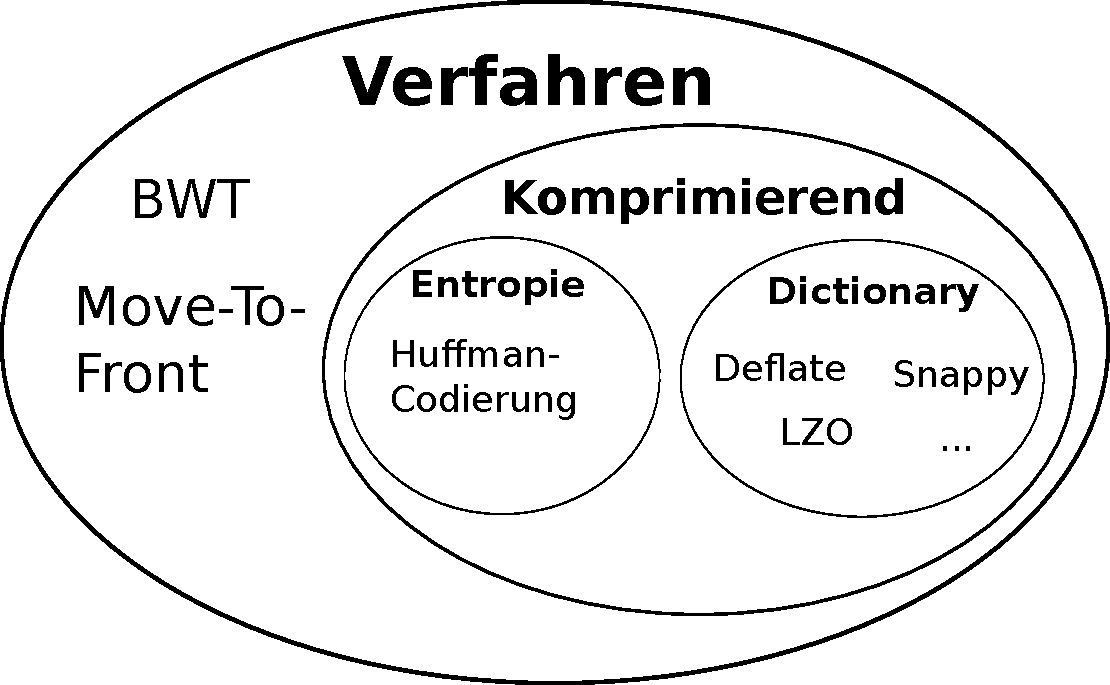
\includegraphics[width=\textwidth]{../Algorithms-Venn.pdf}
\end{frame}

\begin{frame}[allowframebreaks]
 \frametitle{Resultate der Eigenimplementierung}
 \includegraphics[width=\textwidth]{graph/uk-2.pdf}
 \framebreak\\
 \includegraphics[width=\textwidth]{graph/uk-1.pdf}
 \framebreak\\
 \includegraphics[width=\textwidth]{graph/uk-new-calgary.pdf}
 \framebreak\\
 \includegraphics[width=\textwidth]{graph/uk-new-celegans.pdf}
 \framebreak\\
 \includegraphics[width=\textwidth]{graph/uk-time.pdf}
\end{frame}
\begin{frame}[allowframebreaks]
 \frametitle{Diskussion der eigenen Resultate}
 \begin{itemize}
  \item Nur ein kleiner Teil der Resultate konnte hier diskutiert werden
  \item Verbreitete Dictionary-basierte Verfahren wie \textit{Deflate} erzeugen mit BWT größere Dateien als ohne BWT
  \item Kompression von \textit{BWT+MTF+Huffman} erzeugt unter den BWT-Verfahren die besten Größeneinsparungen\\
  \item \textbf{Aber:} Langsame Kompression\\
  \textrightarrow\ Implementierung langsam? Stark Optimierter  Encoder in C++
 \end{itemize}
 \framebreak
 \begin{itemize}
  \item \textbf{bzip2} nutzt den BWT+MTF+Huffman-Algorithmus - gute Kompression, aber vergleichsweise langsam
  \item \textbf{bzip2}-Dekompression ist nicht deutlich schneller als Kompression
  \item BWT+MTF+Huffman erzeugt bei Bioinformatik-Datensätzen nur unwesentlich kleinere Dateien als MTF+Huffman
  \end{itemize}
  \framebreak
  \begin{itemize}
  \item \textbf{Konklusion:} Unmodifizierte BWT ist oft ungeeignet, wenn die Kompressions- oder Dekompressionszeit eine übergeordnete Rolle spielt\\
  \textrightarrow\ BWT-SAP
  \item Mögliche Alternative:\\
  Asymmetrische Kompressionsalgorithmen\\
  \textrightarrow\ Einzelfallentscheidung
 \end{itemize}
\end{frame}

%%%%%% Conclusion
\begin{frame}[allowframebreaks]
 \frametitle{Zusammenfassung}
 \begin{itemize}
  \item Datenkompression ist aufgrund der enormen Datenmengen, die durch Methoden wie High-Throughput-Sequencing entstehen, oftmals notwendig
  \item Verschiedene Algorithmen erreichen verschiedene Kompressionsraten und benötigen unterschiedlich viel Rechenzeit für Kompression und Dekompression
 \end{itemize}
 \framebreak
 \begin{itemize}
  \item Die Burrows-Wheeler-Transformation ist ein Algorithmus, um Zeichenketten besser komprimierbar zu machen
  \item Im beliebten Unix-Programm \textit{bzip2} wird die BWT eingesetzt
  \item BWT-basierte Algorithmen sind nicht für alle Anwendungsfälle
  \end{itemize}
\end{frame}
%%%%%% End
\begin{frame}
 \begin{center}
  {\color{BlueViolet}\large Vielen Dank für eure Aufmerksamkeit!}\\\vspace{1cm}
  Alle Quellen unter \url{https://github.com/ulikoehler/Proseminar}
 \end{center}

\end{frame}

\end{document}
